\section{Noise effects}
To conclude our analysis, in the end we studied the behaviours of the sub-pixel filters varying the noise in the image. As we mentioned in Section \ref{sec:laser-peaks}, the presence of electrical noise in the frames \cite{1334612}, can affect heavily the quality of the peak detection, thus it is a good practice to apply some filters that reduce the weight of this noise during the laser location phase \cite{Naidu1991}. For example, industry experts know that such operations are necessary if you use the \textit{center of mass}: the presence of spikes influences the evaluation of the weighted average. An example of this, is shown in Figure \ref{fig:noise-es}. \\
  \begin{figure}[t!]
    \centering
    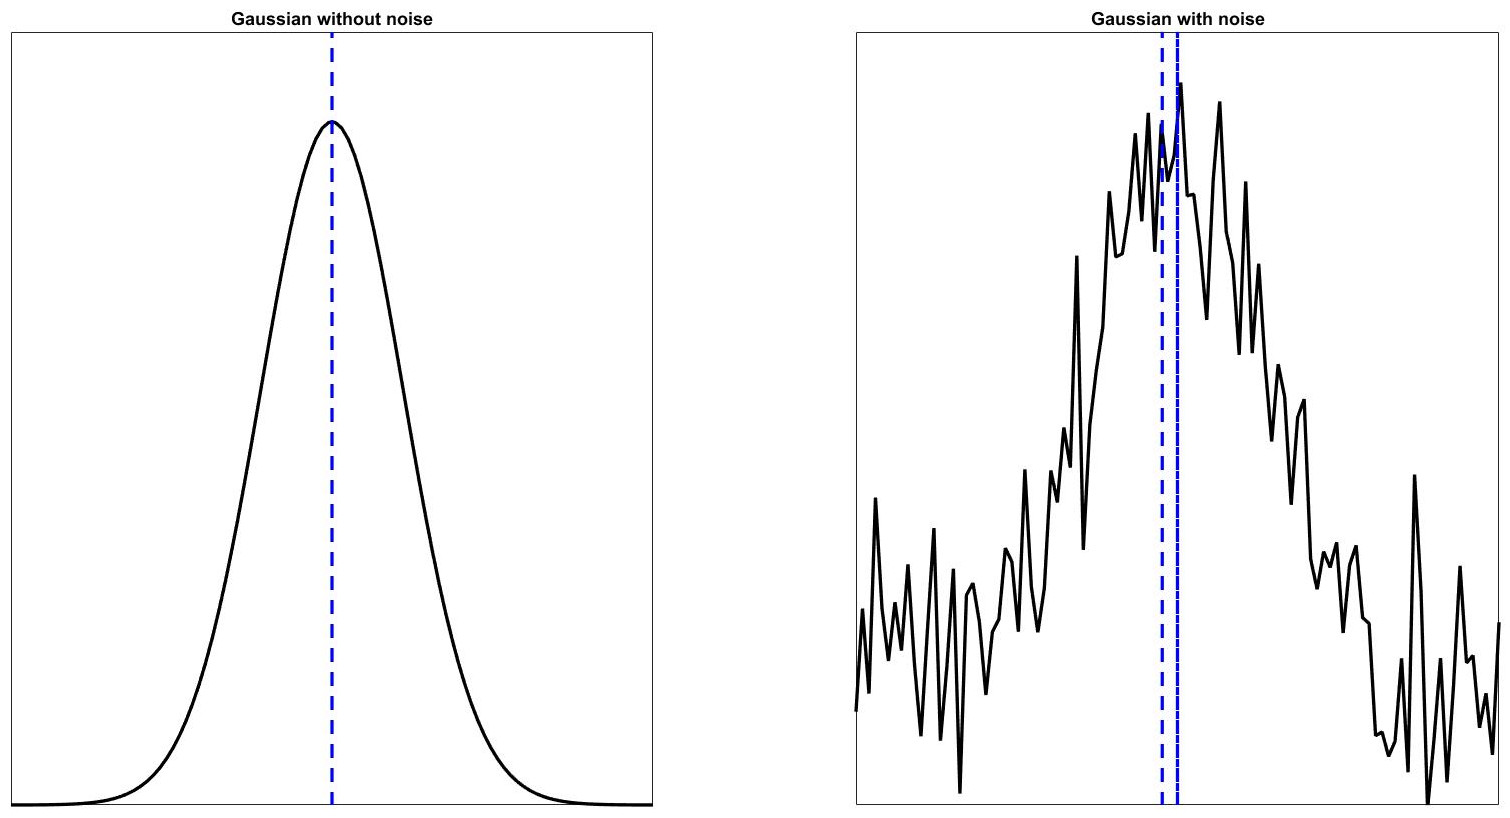
\includegraphics[width=\textwidth]{./images/analysis/noise/electrical.jpg}
    \caption{Effects of noise in peak detection. On the left there is a noise free Gaussian, and the \acs{COM} correctly detect the peak. On the right, the noise moves the location (-.) with respect to the correct one (- -).}
    \label{fig:noise-es}
  \end{figure}
  
As far as we are concerned, we have noticed these problems during the test shown in Section \ref{sec:exp2}. Before reaching the discussed results, we tried to apply different image preprocessing algorithms to increase the precision of the peak localizion. So we saw that when we changed the preprocessing, the final results changed too. In Figure \ref{fig:prep-dima} we reported the model trends for each sub-pixel filter used, varying the image preprocessing algorithms. As we can see, not all algorithms improve the results, on the contrary, sometimes they get worse the final error. In addition, we can see that the trend is different between mobile average and derivatives filters. These observations suggested us that not all filters have the same behaviour. Anyway, these results were obtained from a single system, thus we decided to perform some theoretical tests, in order to control the sources of noise. \\

In the second set of tests, we introduced some noise to the Gaussian, varying its \acs{SNR}. In this way we were able to see how much strong are the sub-pixel algorithms with respect to the noise, and thus to the variations in image conditions. To do that, we varied the \acs{SNR} in the range $\left( 0, 30 \right)$ with step $1$, and repeated the test five times per \acs{SNR} step. The averages of the results are shown in Figures \ref{fig:prep1} and \ref{fig:prep2}. We had to split the trends in two graphics to see better what happens. 

The first thing that caught our attention was the fact that, for high values of \acs{SNR}, the initial hypothesis that $\hat{\delta} \in \left( -\frac{1}{2}, \frac{1}{2} \right)$ with respect to the pixel, is false. The only model that always guarantees the hypothesis, is the \textit{FIR}. Unfortunately, we are not able to model this result mathematically. As we said in the previous chapters, the algorithm used to detects the peak, finds the pixel with the greater value along a row, and then applies on it the sub-pixel filters. If we think of a moment, this is a reasonable hypothesis: so we considered the possibility to go out from the pixel as an error due to the noise in the image.

The second important thing to underline, is the effect of the size of the window. As we have said several times, the window has to be comparable with the width of the Gaussian, however, in presence of noise, the bigger the window is, the bigger is the weight of the noise in the measure. We can see this for both \textit{center of mass} and \textit{B\&R}. Furthermore, in the same point we can notice that the \textit{FIR} filter, that is more robust than the others in presence of noise, becomes the worst. \\

Thus, we can conclude that, from a global point of view, the \textit{FIR} filter is the more robust in presence of noise, and it is the more stable, because of its small variance along noise variation. However, for low noise images \textit{center of mass} and \textit{B\&R} models, allow to reach better results. The \textit{B\&R} is the less stable filter, but as shown in Figure \ref{fig:prep-dima}, it is the less sensible (with the \textit{FIR} filter) to image preprocessing. Finally, as far as the window size is concerned, the rule on Gaussian dimension continues to apply. So, there isn't a filter better than the others: their behaviours strictly depends from the scenario we are working on, and from the preprocess applied to the image. Since these considerations are empirical, we suggest to perform some tests in real conditions before choosing what algorithm use in your application.
  \begin{figure}[b!]
    \centering
    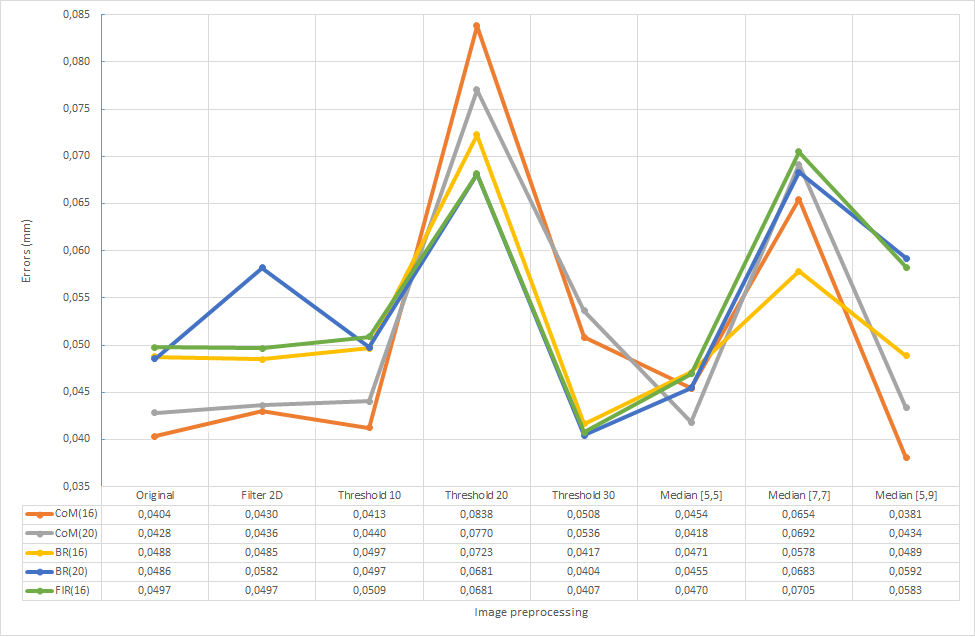
\includegraphics[width=0.95\textwidth]{./images/analysis/noise/preprocessing_dima.png}
    \caption{Variation in the model output changing the image preprocessing.}
    \label{fig:prep-dima}
  \end{figure}
\vfill
  \begin{figure}
    \centering
    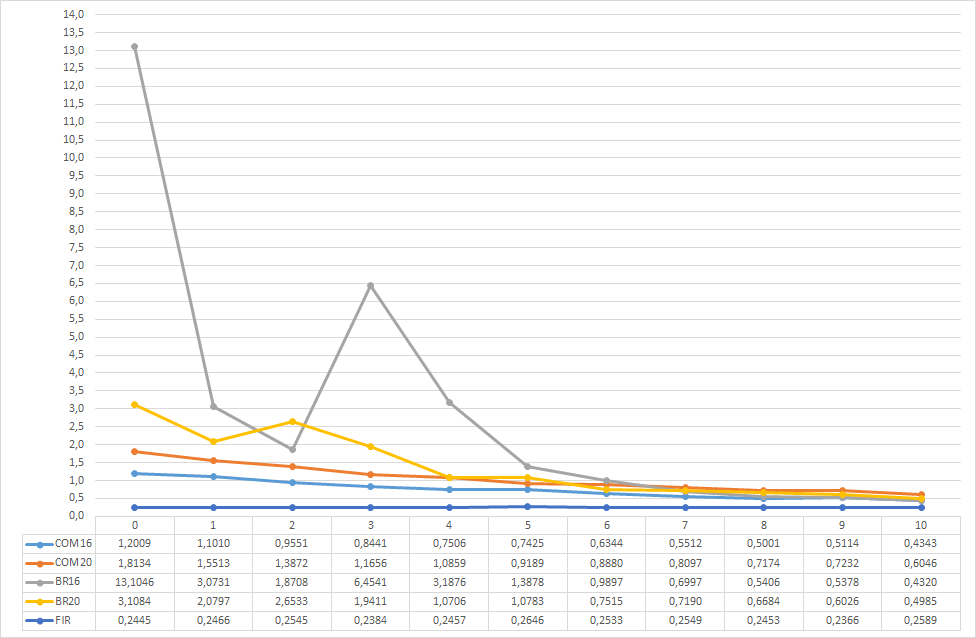
\includegraphics[width=\textwidth]{./images/analysis/noise/prep1.png}
    \caption{Filters' trends for \acs{SNR} in range $\left( 0, 10 \right)$}
    \label{fig:prep1}
  \end{figure}
\vfill
  \begin{figure}[t!]
    \centering
    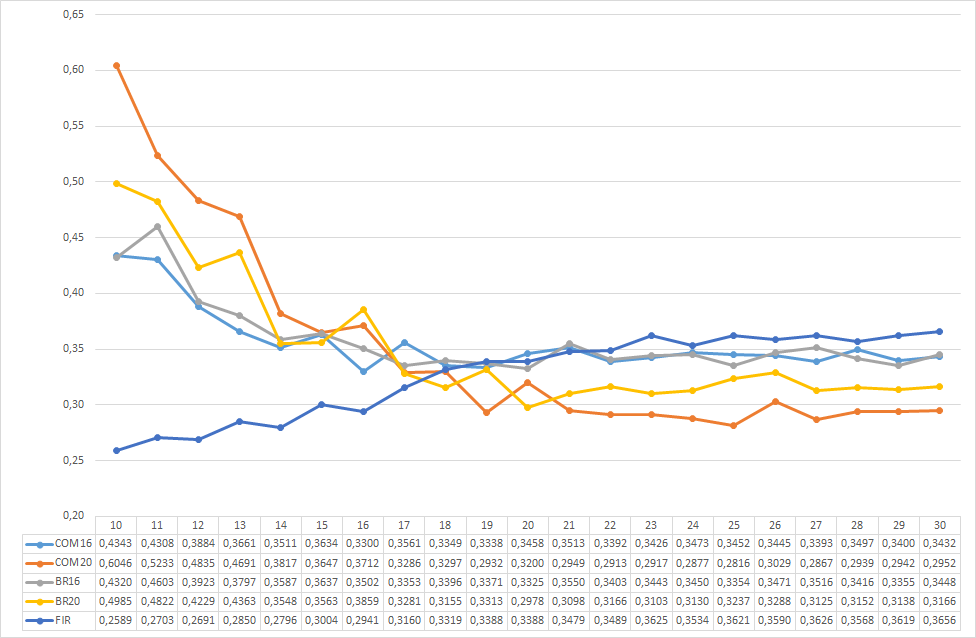
\includegraphics[width=\textwidth]{./images/analysis/noise/prep2.png}
    \caption{Filters' trends for \acs{SNR} in range $\left( 10, 30 \right)$}
    \label{fig:prep2}
  \end{figure}
